% Created by tikzDevice version 0.12.6 on 2024-02-28 09:29:12
% !TEX encoding = UTF-8 Unicode
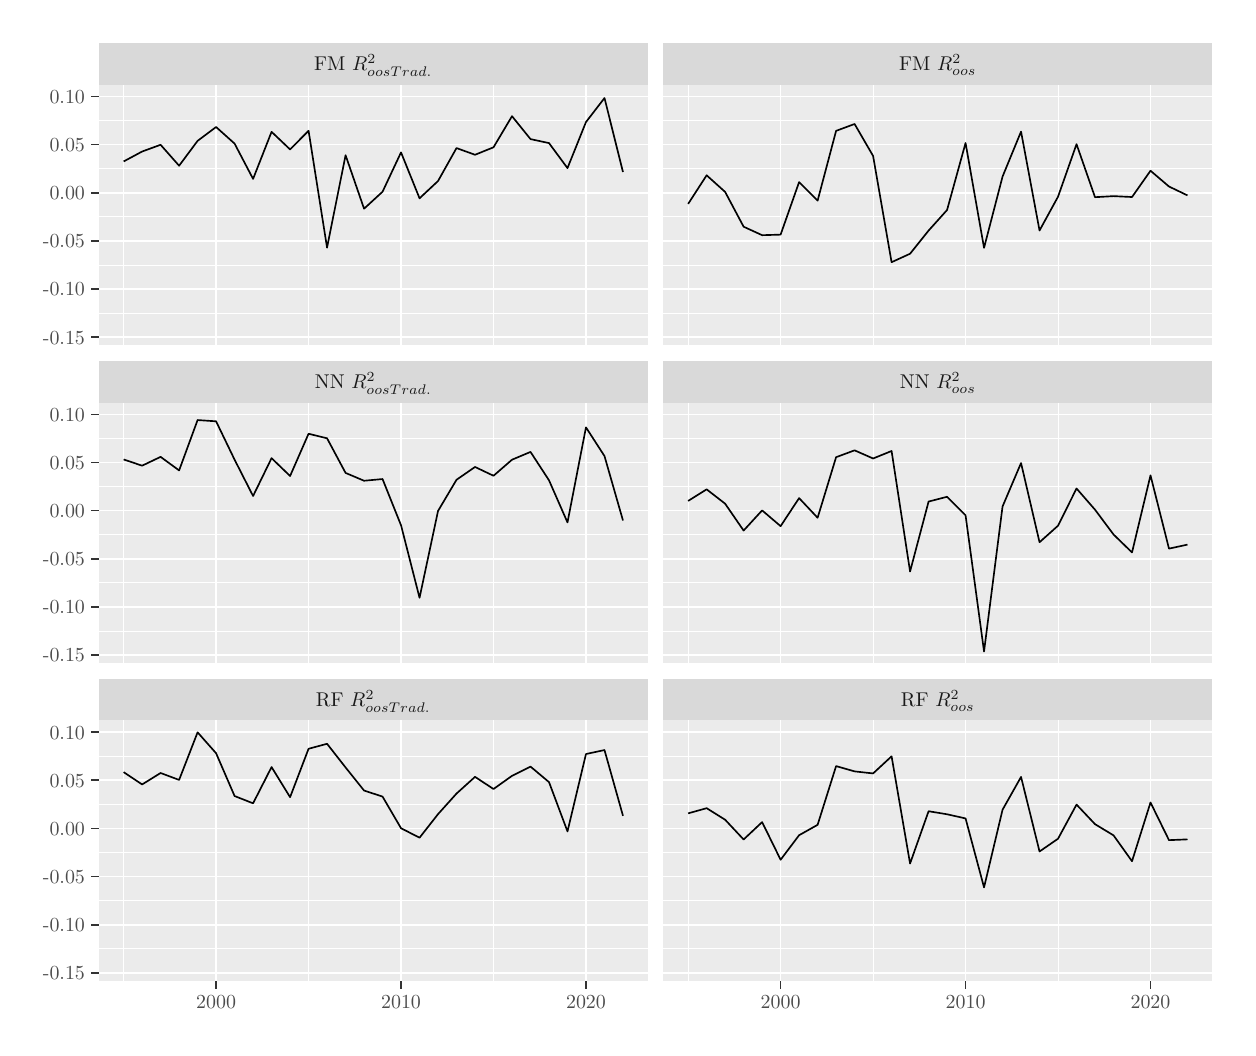
\begin{tikzpicture}[x=1pt,y=1pt]
\definecolor{fillColor}{RGB}{255,255,255}
\path[use as bounding box,fill=fillColor,fill opacity=0.00] (0,0) rectangle (433.62,361.35);
\begin{scope}
\path[clip] (  0.00,  0.00) rectangle (433.62,361.35);
\definecolor{drawColor}{RGB}{255,255,255}
\definecolor{fillColor}{RGB}{255,255,255}

\path[draw=drawColor,line width= 0.6pt,line join=round,line cap=round,fill=fillColor] (  0.00,  0.00) rectangle (433.62,361.35);
\end{scope}
\begin{scope}
\path[clip] ( 25.65,246.50) rectangle (224.13,340.69);
\definecolor{fillColor}{gray}{0.92}

\path[fill=fillColor] ( 25.65,246.50) rectangle (224.13,340.69);
\definecolor{drawColor}{RGB}{255,255,255}

\path[draw=drawColor,line width= 0.3pt,line join=round] ( 25.65,258.21) --
	(224.13,258.21);

\path[draw=drawColor,line width= 0.3pt,line join=round] ( 25.65,275.60) --
	(224.13,275.60);

\path[draw=drawColor,line width= 0.3pt,line join=round] ( 25.65,292.99) --
	(224.13,292.99);

\path[draw=drawColor,line width= 0.3pt,line join=round] ( 25.65,310.38) --
	(224.13,310.38);

\path[draw=drawColor,line width= 0.3pt,line join=round] ( 25.65,327.77) --
	(224.13,327.77);

\path[draw=drawColor,line width= 0.3pt,line join=round] ( 34.67,246.50) --
	( 34.67,340.69);

\path[draw=drawColor,line width= 0.3pt,line join=round] (101.50,246.50) --
	(101.50,340.69);

\path[draw=drawColor,line width= 0.3pt,line join=round] (168.33,246.50) --
	(168.33,340.69);

\path[draw=drawColor,line width= 0.6pt,line join=round] ( 25.65,249.51) --
	(224.13,249.51);

\path[draw=drawColor,line width= 0.6pt,line join=round] ( 25.65,266.90) --
	(224.13,266.90);

\path[draw=drawColor,line width= 0.6pt,line join=round] ( 25.65,284.29) --
	(224.13,284.29);

\path[draw=drawColor,line width= 0.6pt,line join=round] ( 25.65,301.69) --
	(224.13,301.69);

\path[draw=drawColor,line width= 0.6pt,line join=round] ( 25.65,319.08) --
	(224.13,319.08);

\path[draw=drawColor,line width= 0.6pt,line join=round] ( 25.65,336.47) --
	(224.13,336.47);

\path[draw=drawColor,line width= 0.6pt,line join=round] ( 68.08,246.50) --
	( 68.08,340.69);

\path[draw=drawColor,line width= 0.6pt,line join=round] (134.91,246.50) --
	(134.91,340.69);

\path[draw=drawColor,line width= 0.6pt,line join=round] (201.74,246.50) --
	(201.74,340.69);
\definecolor{drawColor}{RGB}{0,0,0}

\path[draw=drawColor,line width= 0.6pt,line join=round] ( 34.67,313.00) --
	( 41.35,316.59) --
	( 48.03,319.03) --
	( 54.72,311.46) --
	( 61.40,320.45) --
	( 68.08,325.45) --
	( 74.77,319.45) --
	( 81.45,306.70) --
	( 88.13,323.71) --
	( 94.82,317.35) --
	(101.50,324.09) --
	(108.18,281.85) --
	(114.87,315.27) --
	(121.55,295.93) --
	(128.23,302.06) --
	(134.91,316.28) --
	(141.60,299.69) --
	(148.28,305.93) --
	(154.96,317.84) --
	(161.65,315.42) --
	(168.33,318.12) --
	(175.01,329.36) --
	(181.70,321.08) --
	(188.38,319.64) --
	(195.06,310.60) --
	(201.74,327.24) --
	(208.43,335.92) --
	(215.11,309.19);
\end{scope}
\begin{scope}
\path[clip] ( 25.65,131.66) rectangle (224.13,225.84);
\definecolor{fillColor}{gray}{0.92}

\path[fill=fillColor] ( 25.65,131.66) rectangle (224.13,225.84);
\definecolor{drawColor}{RGB}{255,255,255}

\path[draw=drawColor,line width= 0.3pt,line join=round] ( 25.65,143.36) --
	(224.13,143.36);

\path[draw=drawColor,line width= 0.3pt,line join=round] ( 25.65,160.75) --
	(224.13,160.75);

\path[draw=drawColor,line width= 0.3pt,line join=round] ( 25.65,178.14) --
	(224.13,178.14);

\path[draw=drawColor,line width= 0.3pt,line join=round] ( 25.65,195.54) --
	(224.13,195.54);

\path[draw=drawColor,line width= 0.3pt,line join=round] ( 25.65,212.93) --
	(224.13,212.93);

\path[draw=drawColor,line width= 0.3pt,line join=round] ( 34.67,131.66) --
	( 34.67,225.84);

\path[draw=drawColor,line width= 0.3pt,line join=round] (101.50,131.66) --
	(101.50,225.84);

\path[draw=drawColor,line width= 0.3pt,line join=round] (168.33,131.66) --
	(168.33,225.84);

\path[draw=drawColor,line width= 0.6pt,line join=round] ( 25.65,134.66) --
	(224.13,134.66);

\path[draw=drawColor,line width= 0.6pt,line join=round] ( 25.65,152.06) --
	(224.13,152.06);

\path[draw=drawColor,line width= 0.6pt,line join=round] ( 25.65,169.45) --
	(224.13,169.45);

\path[draw=drawColor,line width= 0.6pt,line join=round] ( 25.65,186.84) --
	(224.13,186.84);

\path[draw=drawColor,line width= 0.6pt,line join=round] ( 25.65,204.23) --
	(224.13,204.23);

\path[draw=drawColor,line width= 0.6pt,line join=round] ( 25.65,221.62) --
	(224.13,221.62);

\path[draw=drawColor,line width= 0.6pt,line join=round] ( 68.08,131.66) --
	( 68.08,225.84);

\path[draw=drawColor,line width= 0.6pt,line join=round] (134.91,131.66) --
	(134.91,225.84);

\path[draw=drawColor,line width= 0.6pt,line join=round] (201.74,131.66) --
	(201.74,225.84);
\definecolor{drawColor}{RGB}{0,0,0}

\path[draw=drawColor,line width= 0.6pt,line join=round] ( 34.67,205.33) --
	( 41.35,203.07) --
	( 48.03,206.26) --
	( 54.72,201.36) --
	( 61.40,219.56) --
	( 68.08,219.10) --
	( 74.77,205.24) --
	( 81.45,192.11) --
	( 88.13,205.79) --
	( 94.82,199.34) --
	(101.50,214.61) --
	(108.18,212.97) --
	(114.87,200.46) --
	(121.55,197.63) --
	(128.23,198.24) --
	(134.91,181.56) --
	(141.60,155.34) --
	(148.28,186.71) --
	(154.96,197.98) --
	(161.65,202.61) --
	(168.33,199.43) --
	(175.01,205.23) --
	(181.70,208.05) --
	(188.38,197.79) --
	(195.06,182.57) --
	(201.74,216.92) --
	(208.43,206.55) --
	(215.11,183.27);
\end{scope}
\begin{scope}
\path[clip] ( 25.65, 16.81) rectangle (224.13,111.00);
\definecolor{fillColor}{gray}{0.92}

\path[fill=fillColor] ( 25.65, 16.81) rectangle (224.13,111.00);
\definecolor{drawColor}{RGB}{255,255,255}

\path[draw=drawColor,line width= 0.3pt,line join=round] ( 25.65, 28.51) --
	(224.13, 28.51);

\path[draw=drawColor,line width= 0.3pt,line join=round] ( 25.65, 45.90) --
	(224.13, 45.90);

\path[draw=drawColor,line width= 0.3pt,line join=round] ( 25.65, 63.30) --
	(224.13, 63.30);

\path[draw=drawColor,line width= 0.3pt,line join=round] ( 25.65, 80.69) --
	(224.13, 80.69);

\path[draw=drawColor,line width= 0.3pt,line join=round] ( 25.65, 98.08) --
	(224.13, 98.08);

\path[draw=drawColor,line width= 0.3pt,line join=round] ( 34.67, 16.81) --
	( 34.67,111.00);

\path[draw=drawColor,line width= 0.3pt,line join=round] (101.50, 16.81) --
	(101.50,111.00);

\path[draw=drawColor,line width= 0.3pt,line join=round] (168.33, 16.81) --
	(168.33,111.00);

\path[draw=drawColor,line width= 0.6pt,line join=round] ( 25.65, 19.82) --
	(224.13, 19.82);

\path[draw=drawColor,line width= 0.6pt,line join=round] ( 25.65, 37.21) --
	(224.13, 37.21);

\path[draw=drawColor,line width= 0.6pt,line join=round] ( 25.65, 54.60) --
	(224.13, 54.60);

\path[draw=drawColor,line width= 0.6pt,line join=round] ( 25.65, 71.99) --
	(224.13, 71.99);

\path[draw=drawColor,line width= 0.6pt,line join=round] ( 25.65, 89.38) --
	(224.13, 89.38);

\path[draw=drawColor,line width= 0.6pt,line join=round] ( 25.65,106.78) --
	(224.13,106.78);

\path[draw=drawColor,line width= 0.6pt,line join=round] ( 68.08, 16.81) --
	( 68.08,111.00);

\path[draw=drawColor,line width= 0.6pt,line join=round] (134.91, 16.81) --
	(134.91,111.00);

\path[draw=drawColor,line width= 0.6pt,line join=round] (201.74, 16.81) --
	(201.74,111.00);
\definecolor{drawColor}{RGB}{0,0,0}

\path[draw=drawColor,line width= 0.6pt,line join=round] ( 34.67, 92.35) --
	( 41.35, 87.88) --
	( 48.03, 92.03) --
	( 54.72, 89.52) --
	( 61.40,106.72) --
	( 68.08, 99.17) --
	( 74.77, 83.70) --
	( 81.45, 81.07) --
	( 88.13, 94.17) --
	( 94.82, 83.29) --
	(101.50,100.78) --
	(108.18,102.58) --
	(114.87, 94.03) --
	(121.55, 85.69) --
	(128.23, 83.50) --
	(134.91, 72.07) --
	(141.60, 68.64) --
	(148.28, 77.16) --
	(154.96, 84.59) --
	(161.65, 90.63) --
	(168.33, 86.23) --
	(175.01, 91.00) --
	(181.70, 94.34) --
	(188.38, 88.73) --
	(195.06, 70.91) --
	(201.74, 98.88) --
	(208.43,100.32) --
	(215.11, 76.56);
\end{scope}
\begin{scope}
\path[clip] (229.63,246.50) rectangle (428.12,340.69);
\definecolor{fillColor}{gray}{0.92}

\path[fill=fillColor] (229.63,246.50) rectangle (428.12,340.69);
\definecolor{drawColor}{RGB}{255,255,255}

\path[draw=drawColor,line width= 0.3pt,line join=round] (229.63,258.21) --
	(428.12,258.21);

\path[draw=drawColor,line width= 0.3pt,line join=round] (229.63,275.60) --
	(428.12,275.60);

\path[draw=drawColor,line width= 0.3pt,line join=round] (229.63,292.99) --
	(428.12,292.99);

\path[draw=drawColor,line width= 0.3pt,line join=round] (229.63,310.38) --
	(428.12,310.38);

\path[draw=drawColor,line width= 0.3pt,line join=round] (229.63,327.77) --
	(428.12,327.77);

\path[draw=drawColor,line width= 0.3pt,line join=round] (238.66,246.50) --
	(238.66,340.69);

\path[draw=drawColor,line width= 0.3pt,line join=round] (305.49,246.50) --
	(305.49,340.69);

\path[draw=drawColor,line width= 0.3pt,line join=round] (372.32,246.50) --
	(372.32,340.69);

\path[draw=drawColor,line width= 0.6pt,line join=round] (229.63,249.51) --
	(428.12,249.51);

\path[draw=drawColor,line width= 0.6pt,line join=round] (229.63,266.90) --
	(428.12,266.90);

\path[draw=drawColor,line width= 0.6pt,line join=round] (229.63,284.29) --
	(428.12,284.29);

\path[draw=drawColor,line width= 0.6pt,line join=round] (229.63,301.69) --
	(428.12,301.69);

\path[draw=drawColor,line width= 0.6pt,line join=round] (229.63,319.08) --
	(428.12,319.08);

\path[draw=drawColor,line width= 0.6pt,line join=round] (229.63,336.47) --
	(428.12,336.47);

\path[draw=drawColor,line width= 0.6pt,line join=round] (272.07,246.50) --
	(272.07,340.69);

\path[draw=drawColor,line width= 0.6pt,line join=round] (338.90,246.50) --
	(338.90,340.69);

\path[draw=drawColor,line width= 0.6pt,line join=round] (405.73,246.50) --
	(405.73,340.69);
\definecolor{drawColor}{RGB}{0,0,0}

\path[draw=drawColor,line width= 0.6pt,line join=round] (238.66,297.67) --
	(245.34,308.00) --
	(252.02,302.00) --
	(258.70,289.43) --
	(265.39,286.36) --
	(272.07,286.56) --
	(278.75,305.54) --
	(285.44,298.84) --
	(292.12,324.06) --
	(298.80,326.54) --
	(305.49,315.00) --
	(312.17,276.60) --
	(318.85,279.66) --
	(325.54,288.02) --
	(332.22,295.46) --
	(338.90,319.67) --
	(345.58,281.79) --
	(352.27,307.54) --
	(358.95,323.80) --
	(365.63,288.05) --
	(372.32,300.28) --
	(379.00,319.25) --
	(385.68,300.09) --
	(392.37,300.47) --
	(399.05,300.15) --
	(405.73,309.65) --
	(412.41,303.95) --
	(419.10,300.73);
\end{scope}
\begin{scope}
\path[clip] (229.63,131.66) rectangle (428.12,225.84);
\definecolor{fillColor}{gray}{0.92}

\path[fill=fillColor] (229.63,131.66) rectangle (428.12,225.84);
\definecolor{drawColor}{RGB}{255,255,255}

\path[draw=drawColor,line width= 0.3pt,line join=round] (229.63,143.36) --
	(428.12,143.36);

\path[draw=drawColor,line width= 0.3pt,line join=round] (229.63,160.75) --
	(428.12,160.75);

\path[draw=drawColor,line width= 0.3pt,line join=round] (229.63,178.14) --
	(428.12,178.14);

\path[draw=drawColor,line width= 0.3pt,line join=round] (229.63,195.54) --
	(428.12,195.54);

\path[draw=drawColor,line width= 0.3pt,line join=round] (229.63,212.93) --
	(428.12,212.93);

\path[draw=drawColor,line width= 0.3pt,line join=round] (238.66,131.66) --
	(238.66,225.84);

\path[draw=drawColor,line width= 0.3pt,line join=round] (305.49,131.66) --
	(305.49,225.84);

\path[draw=drawColor,line width= 0.3pt,line join=round] (372.32,131.66) --
	(372.32,225.84);

\path[draw=drawColor,line width= 0.6pt,line join=round] (229.63,134.66) --
	(428.12,134.66);

\path[draw=drawColor,line width= 0.6pt,line join=round] (229.63,152.06) --
	(428.12,152.06);

\path[draw=drawColor,line width= 0.6pt,line join=round] (229.63,169.45) --
	(428.12,169.45);

\path[draw=drawColor,line width= 0.6pt,line join=round] (229.63,186.84) --
	(428.12,186.84);

\path[draw=drawColor,line width= 0.6pt,line join=round] (229.63,204.23) --
	(428.12,204.23);

\path[draw=drawColor,line width= 0.6pt,line join=round] (229.63,221.62) --
	(428.12,221.62);

\path[draw=drawColor,line width= 0.6pt,line join=round] (272.07,131.66) --
	(272.07,225.84);

\path[draw=drawColor,line width= 0.6pt,line join=round] (338.90,131.66) --
	(338.90,225.84);

\path[draw=drawColor,line width= 0.6pt,line join=round] (405.73,131.66) --
	(405.73,225.84);
\definecolor{drawColor}{RGB}{0,0,0}

\path[draw=drawColor,line width= 0.6pt,line join=round] (238.66,190.34) --
	(245.34,194.52) --
	(252.02,189.34) --
	(258.70,179.63) --
	(265.39,186.92) --
	(272.07,181.22) --
	(278.75,191.36) --
	(285.44,184.25) --
	(292.12,206.14) --
	(298.80,208.62) --
	(305.49,205.67) --
	(312.17,208.38) --
	(318.85,164.84) --
	(325.54,190.10) --
	(332.22,191.84) --
	(338.90,185.15) --
	(345.58,135.94) --
	(352.27,188.34) --
	(358.95,204.03) --
	(365.63,175.41) --
	(372.32,181.39) --
	(379.00,194.83) --
	(385.68,187.17) --
	(392.37,178.21) --
	(399.05,171.72) --
	(405.73,199.58) --
	(412.41,173.10) --
	(419.10,174.55);
\end{scope}
\begin{scope}
\path[clip] (229.63, 16.81) rectangle (428.12,111.00);
\definecolor{fillColor}{gray}{0.92}

\path[fill=fillColor] (229.63, 16.81) rectangle (428.12,111.00);
\definecolor{drawColor}{RGB}{255,255,255}

\path[draw=drawColor,line width= 0.3pt,line join=round] (229.63, 28.51) --
	(428.12, 28.51);

\path[draw=drawColor,line width= 0.3pt,line join=round] (229.63, 45.90) --
	(428.12, 45.90);

\path[draw=drawColor,line width= 0.3pt,line join=round] (229.63, 63.30) --
	(428.12, 63.30);

\path[draw=drawColor,line width= 0.3pt,line join=round] (229.63, 80.69) --
	(428.12, 80.69);

\path[draw=drawColor,line width= 0.3pt,line join=round] (229.63, 98.08) --
	(428.12, 98.08);

\path[draw=drawColor,line width= 0.3pt,line join=round] (238.66, 16.81) --
	(238.66,111.00);

\path[draw=drawColor,line width= 0.3pt,line join=round] (305.49, 16.81) --
	(305.49,111.00);

\path[draw=drawColor,line width= 0.3pt,line join=round] (372.32, 16.81) --
	(372.32,111.00);

\path[draw=drawColor,line width= 0.6pt,line join=round] (229.63, 19.82) --
	(428.12, 19.82);

\path[draw=drawColor,line width= 0.6pt,line join=round] (229.63, 37.21) --
	(428.12, 37.21);

\path[draw=drawColor,line width= 0.6pt,line join=round] (229.63, 54.60) --
	(428.12, 54.60);

\path[draw=drawColor,line width= 0.6pt,line join=round] (229.63, 71.99) --
	(428.12, 71.99);

\path[draw=drawColor,line width= 0.6pt,line join=round] (229.63, 89.38) --
	(428.12, 89.38);

\path[draw=drawColor,line width= 0.6pt,line join=round] (229.63,106.78) --
	(428.12,106.78);

\path[draw=drawColor,line width= 0.6pt,line join=round] (272.07, 16.81) --
	(272.07,111.00);

\path[draw=drawColor,line width= 0.6pt,line join=round] (338.90, 16.81) --
	(338.90,111.00);

\path[draw=drawColor,line width= 0.6pt,line join=round] (405.73, 16.81) --
	(405.73,111.00);
\definecolor{drawColor}{RGB}{0,0,0}

\path[draw=drawColor,line width= 0.6pt,line join=round] (238.66, 77.44) --
	(245.34, 79.31) --
	(252.02, 75.14) --
	(258.70, 68.00) --
	(265.39, 74.28) --
	(272.07, 60.68) --
	(278.75, 69.54) --
	(285.44, 73.30) --
	(292.12, 94.52) --
	(298.80, 92.61) --
	(305.49, 91.87) --
	(312.17, 98.05) --
	(318.85, 59.31) --
	(325.54, 78.21) --
	(332.22, 77.11) --
	(338.90, 75.61) --
	(345.58, 50.68) --
	(352.27, 78.76) --
	(358.95, 90.61) --
	(365.63, 63.66) --
	(372.32, 68.28) --
	(379.00, 80.61) --
	(385.68, 73.54) --
	(392.37, 69.49) --
	(399.05, 60.15) --
	(405.73, 81.37) --
	(412.41, 67.76) --
	(419.10, 68.04);
\end{scope}
\begin{scope}
\path[clip] ( 25.65,111.00) rectangle (224.13,126.16);
\definecolor{fillColor}{gray}{0.85}

\path[fill=fillColor] ( 25.65,111.00) rectangle (224.13,126.16);
\definecolor{drawColor}{gray}{0.10}

\node[text=drawColor,anchor=base,inner sep=0pt, outer sep=0pt, scale=  0.72] at (124.89,116.10) {RF $R^2_{oos  Trad.}$};
\end{scope}
\begin{scope}
\path[clip] (229.63,111.00) rectangle (428.12,126.16);
\definecolor{fillColor}{gray}{0.85}

\path[fill=fillColor] (229.63,111.00) rectangle (428.12,126.16);
\definecolor{drawColor}{gray}{0.10}

\node[text=drawColor,anchor=base,inner sep=0pt, outer sep=0pt, scale=  0.72] at (328.88,116.10) {RF $R^2_{oos}$};
\end{scope}
\begin{scope}
\path[clip] ( 25.65,225.84) rectangle (224.13,241.00);
\definecolor{fillColor}{gray}{0.85}

\path[fill=fillColor] ( 25.65,225.84) rectangle (224.13,241.00);
\definecolor{drawColor}{gray}{0.10}

\node[text=drawColor,anchor=base,inner sep=0pt, outer sep=0pt, scale=  0.72] at (124.89,230.94) {NN $R^2_{oos  Trad.}$};
\end{scope}
\begin{scope}
\path[clip] (229.63,225.84) rectangle (428.12,241.00);
\definecolor{fillColor}{gray}{0.85}

\path[fill=fillColor] (229.63,225.84) rectangle (428.12,241.00);
\definecolor{drawColor}{gray}{0.10}

\node[text=drawColor,anchor=base,inner sep=0pt, outer sep=0pt, scale=  0.72] at (328.88,230.94) {NN $R^2_{oos}$};
\end{scope}
\begin{scope}
\path[clip] ( 25.65,340.69) rectangle (224.13,355.85);
\definecolor{fillColor}{gray}{0.85}

\path[fill=fillColor] ( 25.65,340.69) rectangle (224.13,355.85);
\definecolor{drawColor}{gray}{0.10}

\node[text=drawColor,anchor=base,inner sep=0pt, outer sep=0pt, scale=  0.72] at (124.89,345.79) {FM $R^2_{oos  Trad.}$};
\end{scope}
\begin{scope}
\path[clip] (229.63,340.69) rectangle (428.12,355.85);
\definecolor{fillColor}{gray}{0.85}

\path[fill=fillColor] (229.63,340.69) rectangle (428.12,355.85);
\definecolor{drawColor}{gray}{0.10}

\node[text=drawColor,anchor=base,inner sep=0pt, outer sep=0pt, scale=  0.72] at (328.88,345.79) {FM $R^2_{oos}$};
\end{scope}
\begin{scope}
\path[clip] (  0.00,  0.00) rectangle (433.62,361.35);
\definecolor{drawColor}{gray}{0.20}

\path[draw=drawColor,line width= 0.6pt,line join=round] ( 68.08, 14.06) --
	( 68.08, 16.81);

\path[draw=drawColor,line width= 0.6pt,line join=round] (134.91, 14.06) --
	(134.91, 16.81);

\path[draw=drawColor,line width= 0.6pt,line join=round] (201.74, 14.06) --
	(201.74, 16.81);
\end{scope}
\begin{scope}
\path[clip] (  0.00,  0.00) rectangle (433.62,361.35);
\definecolor{drawColor}{gray}{0.30}

\node[text=drawColor,anchor=base,inner sep=0pt, outer sep=0pt, scale=  0.72] at ( 68.08,  6.90) {2000};

\node[text=drawColor,anchor=base,inner sep=0pt, outer sep=0pt, scale=  0.72] at (134.91,  6.90) {2010};

\node[text=drawColor,anchor=base,inner sep=0pt, outer sep=0pt, scale=  0.72] at (201.74,  6.90) {2020};
\end{scope}
\begin{scope}
\path[clip] (  0.00,  0.00) rectangle (433.62,361.35);
\definecolor{drawColor}{gray}{0.20}

\path[draw=drawColor,line width= 0.6pt,line join=round] (272.07, 14.06) --
	(272.07, 16.81);

\path[draw=drawColor,line width= 0.6pt,line join=round] (338.90, 14.06) --
	(338.90, 16.81);

\path[draw=drawColor,line width= 0.6pt,line join=round] (405.73, 14.06) --
	(405.73, 16.81);
\end{scope}
\begin{scope}
\path[clip] (  0.00,  0.00) rectangle (433.62,361.35);
\definecolor{drawColor}{gray}{0.30}

\node[text=drawColor,anchor=base,inner sep=0pt, outer sep=0pt, scale=  0.72] at (272.07,  6.90) {2000};

\node[text=drawColor,anchor=base,inner sep=0pt, outer sep=0pt, scale=  0.72] at (338.90,  6.90) {2010};

\node[text=drawColor,anchor=base,inner sep=0pt, outer sep=0pt, scale=  0.72] at (405.73,  6.90) {2020};
\end{scope}
\begin{scope}
\path[clip] (  0.00,  0.00) rectangle (433.62,361.35);
\definecolor{drawColor}{gray}{0.30}

\node[text=drawColor,anchor=base east,inner sep=0pt, outer sep=0pt, scale=  0.72] at ( 20.70,247.03) {-0.15};

\node[text=drawColor,anchor=base east,inner sep=0pt, outer sep=0pt, scale=  0.72] at ( 20.70,264.42) {-0.10};

\node[text=drawColor,anchor=base east,inner sep=0pt, outer sep=0pt, scale=  0.72] at ( 20.70,281.82) {-0.05};

\node[text=drawColor,anchor=base east,inner sep=0pt, outer sep=0pt, scale=  0.72] at ( 20.70,299.21) {0.00};

\node[text=drawColor,anchor=base east,inner sep=0pt, outer sep=0pt, scale=  0.72] at ( 20.70,316.60) {0.05};

\node[text=drawColor,anchor=base east,inner sep=0pt, outer sep=0pt, scale=  0.72] at ( 20.70,333.99) {0.10};
\end{scope}
\begin{scope}
\path[clip] (  0.00,  0.00) rectangle (433.62,361.35);
\definecolor{drawColor}{gray}{0.20}

\path[draw=drawColor,line width= 0.6pt,line join=round] ( 22.90,249.51) --
	( 25.65,249.51);

\path[draw=drawColor,line width= 0.6pt,line join=round] ( 22.90,266.90) --
	( 25.65,266.90);

\path[draw=drawColor,line width= 0.6pt,line join=round] ( 22.90,284.29) --
	( 25.65,284.29);

\path[draw=drawColor,line width= 0.6pt,line join=round] ( 22.90,301.69) --
	( 25.65,301.69);

\path[draw=drawColor,line width= 0.6pt,line join=round] ( 22.90,319.08) --
	( 25.65,319.08);

\path[draw=drawColor,line width= 0.6pt,line join=round] ( 22.90,336.47) --
	( 25.65,336.47);
\end{scope}
\begin{scope}
\path[clip] (  0.00,  0.00) rectangle (433.62,361.35);
\definecolor{drawColor}{gray}{0.30}

\node[text=drawColor,anchor=base east,inner sep=0pt, outer sep=0pt, scale=  0.72] at ( 20.70,132.18) {-0.15};

\node[text=drawColor,anchor=base east,inner sep=0pt, outer sep=0pt, scale=  0.72] at ( 20.70,149.58) {-0.10};

\node[text=drawColor,anchor=base east,inner sep=0pt, outer sep=0pt, scale=  0.72] at ( 20.70,166.97) {-0.05};

\node[text=drawColor,anchor=base east,inner sep=0pt, outer sep=0pt, scale=  0.72] at ( 20.70,184.36) {0.00};

\node[text=drawColor,anchor=base east,inner sep=0pt, outer sep=0pt, scale=  0.72] at ( 20.70,201.75) {0.05};

\node[text=drawColor,anchor=base east,inner sep=0pt, outer sep=0pt, scale=  0.72] at ( 20.70,219.14) {0.10};
\end{scope}
\begin{scope}
\path[clip] (  0.00,  0.00) rectangle (433.62,361.35);
\definecolor{drawColor}{gray}{0.20}

\path[draw=drawColor,line width= 0.6pt,line join=round] ( 22.90,134.66) --
	( 25.65,134.66);

\path[draw=drawColor,line width= 0.6pt,line join=round] ( 22.90,152.06) --
	( 25.65,152.06);

\path[draw=drawColor,line width= 0.6pt,line join=round] ( 22.90,169.45) --
	( 25.65,169.45);

\path[draw=drawColor,line width= 0.6pt,line join=round] ( 22.90,186.84) --
	( 25.65,186.84);

\path[draw=drawColor,line width= 0.6pt,line join=round] ( 22.90,204.23) --
	( 25.65,204.23);

\path[draw=drawColor,line width= 0.6pt,line join=round] ( 22.90,221.62) --
	( 25.65,221.62);
\end{scope}
\begin{scope}
\path[clip] (  0.00,  0.00) rectangle (433.62,361.35);
\definecolor{drawColor}{gray}{0.30}

\node[text=drawColor,anchor=base east,inner sep=0pt, outer sep=0pt, scale=  0.72] at ( 20.70, 17.34) {-0.15};

\node[text=drawColor,anchor=base east,inner sep=0pt, outer sep=0pt, scale=  0.72] at ( 20.70, 34.73) {-0.10};

\node[text=drawColor,anchor=base east,inner sep=0pt, outer sep=0pt, scale=  0.72] at ( 20.70, 52.12) {-0.05};

\node[text=drawColor,anchor=base east,inner sep=0pt, outer sep=0pt, scale=  0.72] at ( 20.70, 69.51) {0.00};

\node[text=drawColor,anchor=base east,inner sep=0pt, outer sep=0pt, scale=  0.72] at ( 20.70, 86.90) {0.05};

\node[text=drawColor,anchor=base east,inner sep=0pt, outer sep=0pt, scale=  0.72] at ( 20.70,104.30) {0.10};
\end{scope}
\begin{scope}
\path[clip] (  0.00,  0.00) rectangle (433.62,361.35);
\definecolor{drawColor}{gray}{0.20}

\path[draw=drawColor,line width= 0.6pt,line join=round] ( 22.90, 19.82) --
	( 25.65, 19.82);

\path[draw=drawColor,line width= 0.6pt,line join=round] ( 22.90, 37.21) --
	( 25.65, 37.21);

\path[draw=drawColor,line width= 0.6pt,line join=round] ( 22.90, 54.60) --
	( 25.65, 54.60);

\path[draw=drawColor,line width= 0.6pt,line join=round] ( 22.90, 71.99) --
	( 25.65, 71.99);

\path[draw=drawColor,line width= 0.6pt,line join=round] ( 22.90, 89.38) --
	( 25.65, 89.38);

\path[draw=drawColor,line width= 0.6pt,line join=round] ( 22.90,106.78) --
	( 25.65,106.78);
\end{scope}
\end{tikzpicture}
